\chapter{信誉算法的参数调优与特征分析}
本章使用上述原型系统,针对信誉算法各项参数取值对于系统敏感度、精确度的影响设计了实验。实验对车辆行驶场景进行简化与模拟,通过构造多种不同情况下的交通状态与车辆交互结果,完成对信誉评估算法中各项参数的特征分析和结果调优。

\section{测试方法}
在本节的模拟测试中,笔者将实际交通地形与车辆行驶状况进行了简化,构造沿经线或纬线分布、长度一致、呈田字格式排列的道路,使模拟的目标车辆在道路上匀速行驶,并以相同的时间间隔更新自己的位置信息。

在下文所述的模拟实验中,目标车辆每隔1秒种更新一次自己的位置,走完田字格道路的一条单位边共需100秒,即一条道路上均匀分布行驶轨迹的100个数据点。生成的原始数据点坐标由经纬度表示,经过转换计算可知,两个相邻数据点之间间隔约为10米;在以下实验中,为便于计算与表述,称该长度为单位距离,称田字格道路的一条单位边为一条道路。

因为该实验只对目标车辆的信誉变化进行追踪,因此在邻居车辆的模拟数据生成时,仅生成两辆车交互成功时邻居车辆的坐标点,而不对其进行动态的轨迹模拟。

\section{参数设计与分析}
本节将根据模拟测试的结果,对第2章中信誉算法的各个参数取值进行调优,主要评价内容及分析指标如表~\ref{tab:params}所示。

\begin{table}
  \centering
  \caption{测试参数及评价指标}
  \begin{tabular}{ll}
    \toprule
    测试参数          & 评价指标                         \\
    \midrule
    时间衰减系数的缩放参数$\delta$   & 信誉变化敏感度 \\
    位置验证权重参数$\theta_s$、$\theta_f$   & 信誉变化趋势、对错误结果的敏感度                     \\
    消息传播的距离衰减系数$\gamma$、消息可信区域划分   &    评价结果波动性    \\
    \bottomrule
  \end{tabular}
  \label{tab:params}
\end{table}

\subsection{时间衰减参数}
本实验基于真实的交通状况,对道路上的车辆分布进行了两种模拟:在一条道路上车辆均匀分布,或者在道路的前半部分均匀、相对稀疏地分布,在靠近道路末尾处车辆密集分布。两种情况分别模拟了车辆正常行驶以及在路口处进行等待两种情况。具体地,两种模拟情况中一条道路上都有20台邻近车辆,其中正常行驶情况下20辆车在道路上呈随机、均匀分布,路口等待情况下10辆车在道路前80\%部分随机分布、10辆车在后20\%部分随机分布。

图~\ref{fig:decay}展示了时间衰减系数的缩放参数$\delta$在不同取值下,目标车辆在一条道路上完成随机生成的20次位置验证所对应的信誉曲线变化。其中,各组实验的位置验证总成功率均为80\%,每张子图中的两条曲线分别对应车辆均匀分布、路口处密集分布两种情况。

\begin{figure}
  \centering
  \subcaptionbox{$\delta=0.1$\label{fig:decay01}}
    {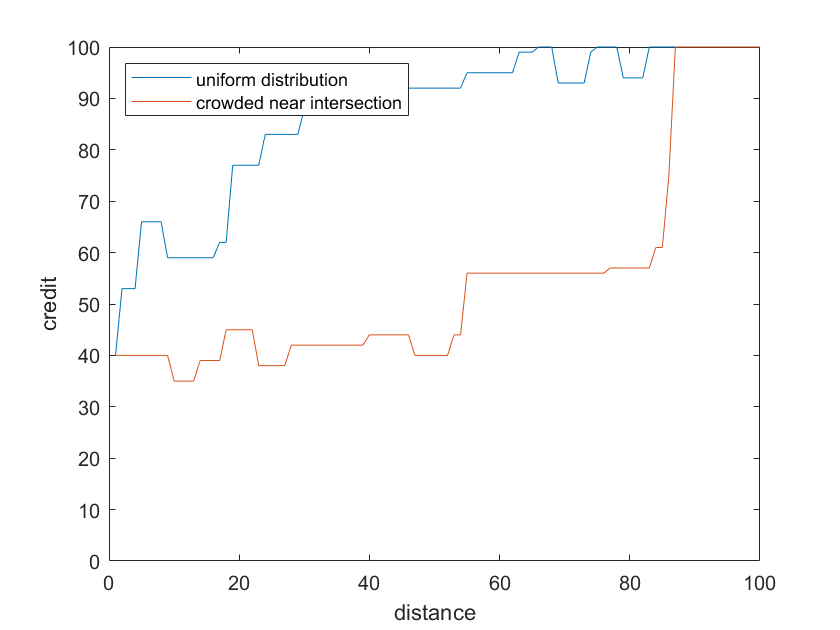
\includegraphics[width=0.49\linewidth]{figures/decay01.png}}
  \subcaptionbox{$\delta=0.2$\label{fig:decay02}}
    {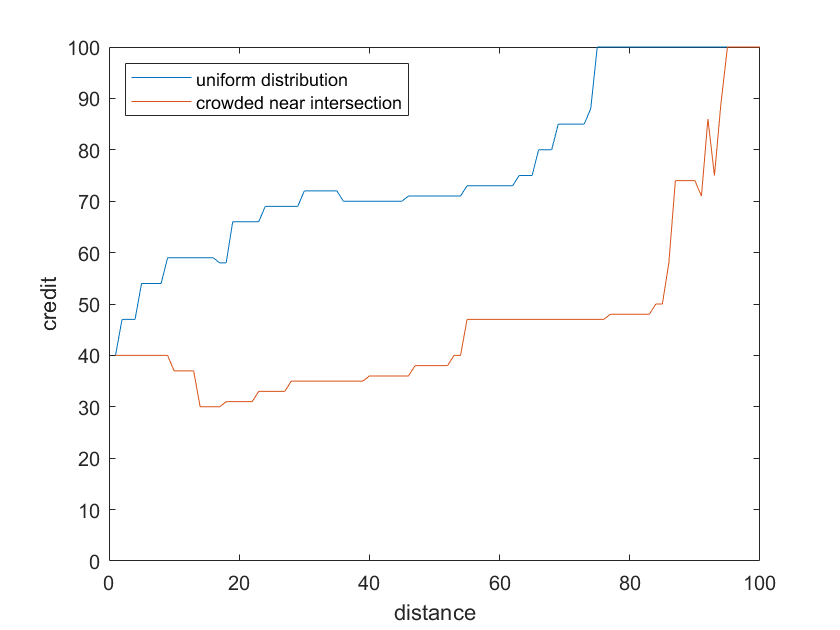
\includegraphics[width=0.49\linewidth]{figures/decay02.png}}
    \subcaptionbox{$\delta=0.3$\label{fig:decay03}}
    {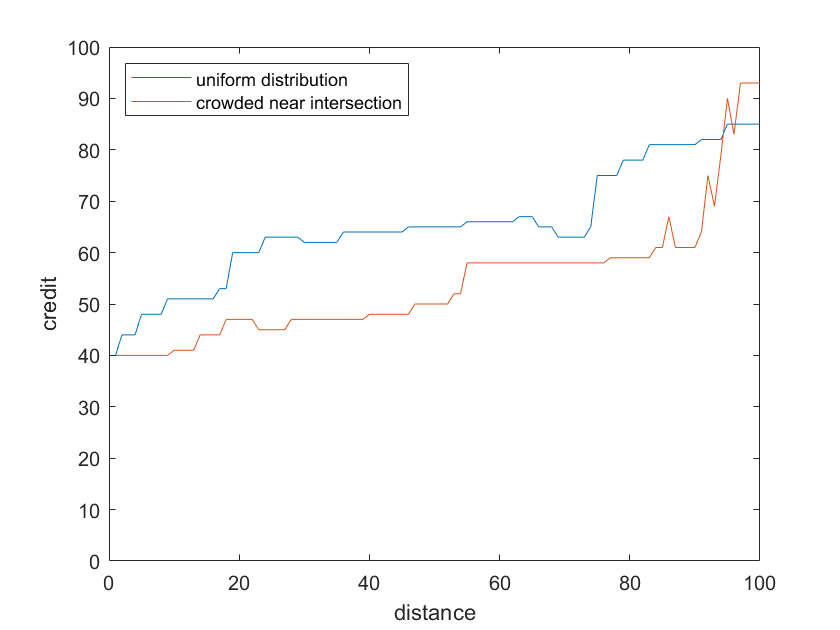
\includegraphics[width=0.49\linewidth]{figures/decay03.png}}
    \subcaptionbox{$\delta=0.5$\label{fig:decay05}}
    {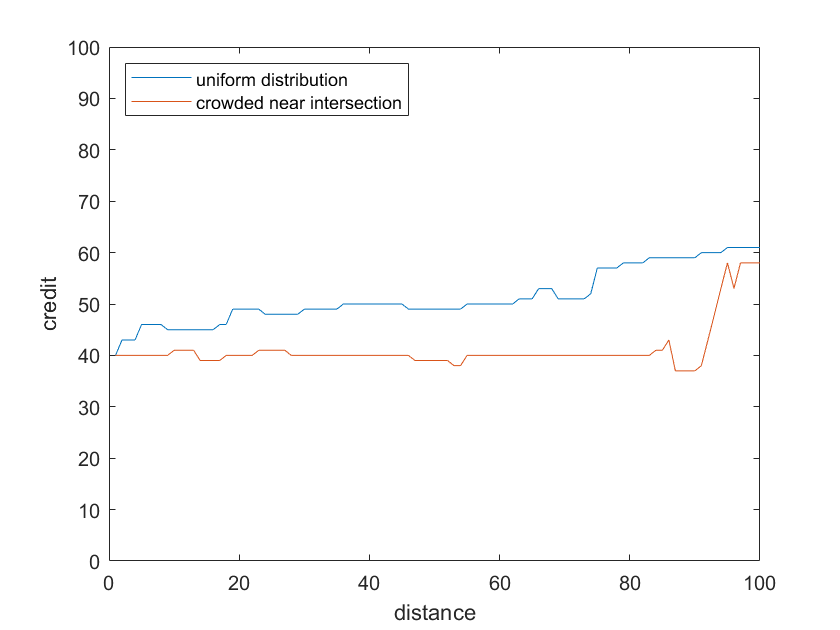
\includegraphics[width=0.49\linewidth]{figures/decay05.png}}
  \caption{不同$\delta$值在两种车辆分布模式下的信誉曲线}
  \label{fig:decay}
\end{figure}

可以看到,在位置验证成功率较高的条件下,各组实验中目标车辆的信誉曲线基本都呈上升趋势,但是数值的波动对数据提交时间的敏感度相差很大;尤其是当有多辆车在路口处密集分布时,过小的缩放参数与频繁的数据提交非常容易导致信誉值的暴涨或暴跌,而这一现象可能只需要两到三次集中的位置验证结果就能发生。相反地,同样可以看到,当该缩放参数取值过大时,目标车辆在正常行驶的过程中则很难产生足够明显的信誉值变化,必须依靠足够密集的数据才能使其得到实质上的提升。该结果一部分是由于智能合约上对数据计算的限制,系统最终会将信誉偏移值归约为整数,如果对数据提交时间的缩放系数不够小,该计算结果很容易会被削减至0,使得交互结果对信誉的影响完全得不到体现。

图~\ref{fig:decay_comp}更加明显地体现了参数$\delta$的取值对系统敏感度的影响。本组实验选取了不同的位置验证成功率和邻近车辆分布,对于每种情况都随机生成同一组交互结果,每个子图展示了在该组交互结果下参数不同取值对信誉曲线的影响。可以看到,每组实验中信誉曲线的整体走势基本一致,但是数据增减的幅度差别很大。考虑到需要让系统对交互结果拥有足够的敏感度,同时避免车辆密集的情况下出现极端的波动,经过多次对比试验,确定$\delta=0.2$为合适的缩放值。

\begin{figure}
  \centering
  \subcaptionbox{验证成功率80\%,均匀分布\label{fig:decaye80}}
    {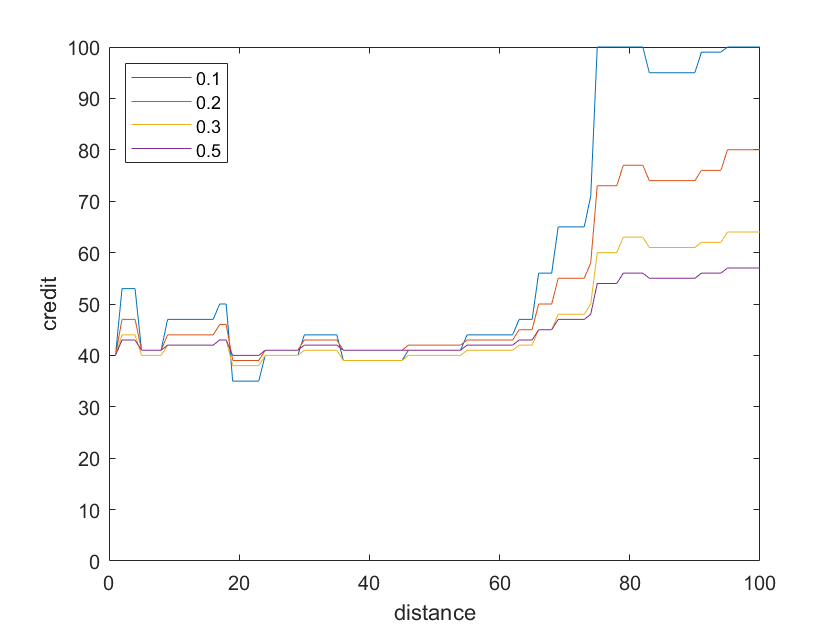
\includegraphics[width=0.49\linewidth]{figures/decay_even_80.png}}
  \subcaptionbox{验证成功率60\%,均匀分布\label{fig:decaye60}}
    {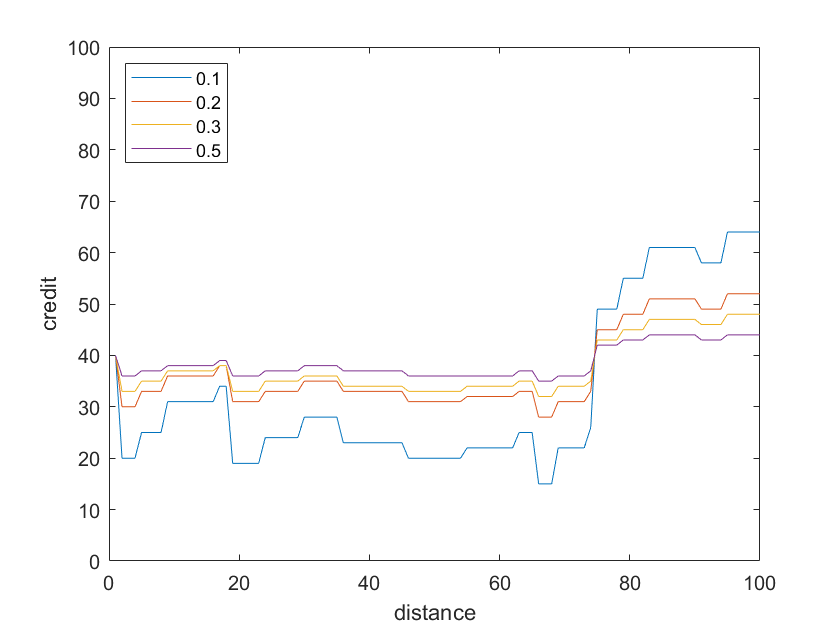
\includegraphics[width=0.49\linewidth]{figures/decay_even_60.png}}
    \subcaptionbox{验证成功率80\%,路口密集\label{fig:decayu80}}
    {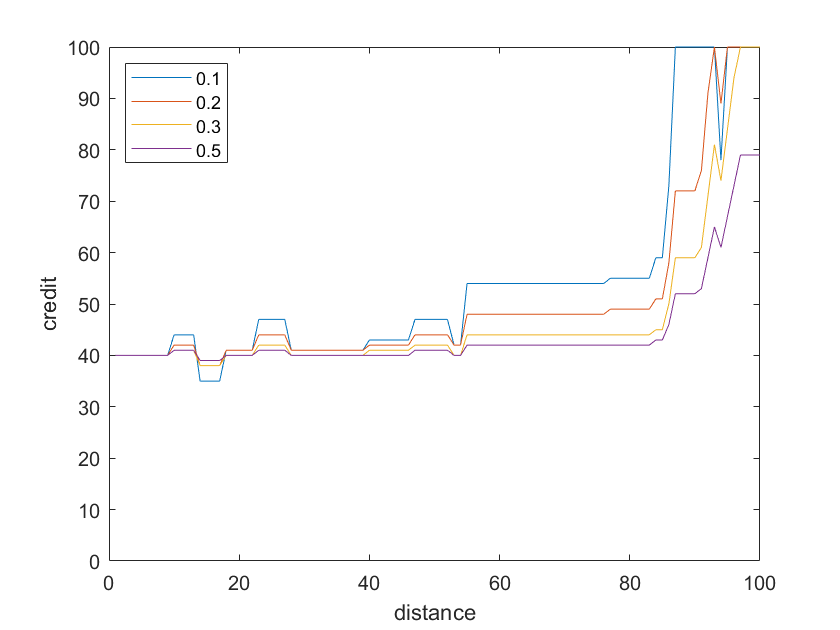
\includegraphics[width=0.49\linewidth]{figures/decay_ueven_80.png}}
    \subcaptionbox{验证成功率60\%,路口密集\label{fig:decayu60}}
    {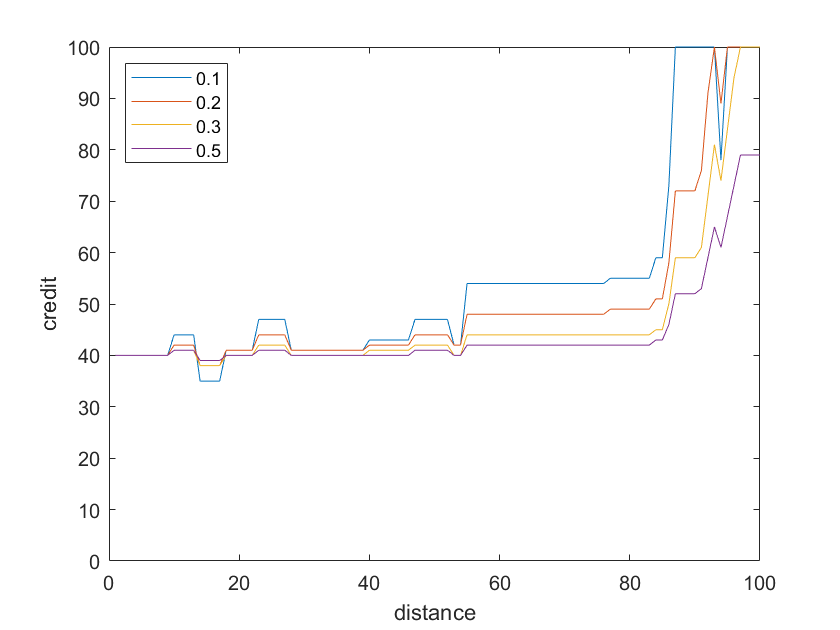
\includegraphics[width=0.49\linewidth]{figures/decay_ueven_80.png}}
  \caption{不同$\delta$值在同一组交互结果下的信誉曲线}
  \label{fig:decay_comp}
\end{figure}

\subsection{基于位置验证的信誉计算参数}
在对位置验证结果的信誉计算中,验证结果成功、失败分别对应一个权重参数$\theta_s$、$\theta_f$。本节的实验中,首先对两参数绝对值的大小关系进行讨论,然后再针对具体取值做进一步的实验。

对于车辆在路口处密集分布的情况,假设总体的位置验证成功率为80\%、60\%、40\%,对这三种场景分别随机生成一组验证结果,具有不同大小关系的权重参数在各组验证结果下所展现的信誉曲线如图4.3所示。三张子图显示的结果相对较为统一,每张图中三条曲线由上至下,对于位置验证失败情况的敏感度依次增强。

值得注意的是,虽然测试中各组参数对每次位置验证结果单独的响应是基本一致的,但是在目标车辆行驶完一条道路后信誉值在整体上的变化有所不同。这一点在图~\ref{fig:theta_comp}b中体现得尤为明显:在位置验证成功率为60\%的情况下,第一组参数对应的曲线最终达到了信誉最大值,但是对于同样的验证结果,第三组参数对应的信誉则基本一直维持在较低的不可信水平。

\begin{figure}
  \centering
  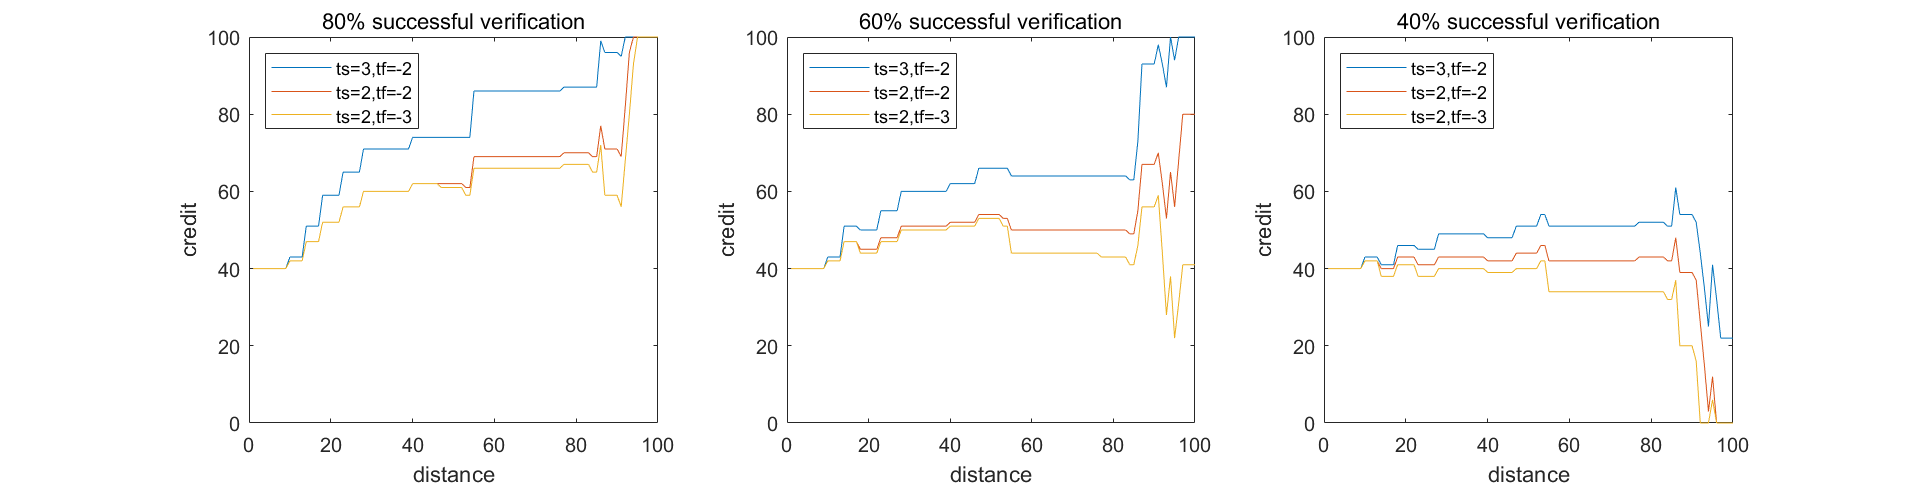
\includegraphics[width=1\linewidth]{figures/theta_comp_total.png}
  \caption{给定验证成功率时,权重参数不同数量关系对应的信誉曲线}
  \label{fig:theta_comp}
\end{figure}

基于上述实验,最终选择两参数的大小关系为$\theta_s<\theta_f$,是考虑到判定一个车辆可信应当需要其在一定程度上持续、稳定地与其他车辆完成成功的位置验证,相对地,验证失败对应的惩罚应当更大,否则仅靠少数成功结果就能很快弥补信誉值的缺失是不合理的。

在确定参数的大小关系后,笔者进一步选取了几组不同的参数取值,重复上述实验。图~\ref{fig:theta_num}展示了各组参数对应的信誉变化结果。通过多次对比实验,最终确定权重参数取值$\theta_{s}=2,\theta_{f}=-3$,使得数据波动能够保持在合理范围内,同时确保每一次计算信誉偏移值时,当次验证结果的影响力能够得到充分的体现,而不被历史数据掩盖。

\begin{figure}
  \centering
  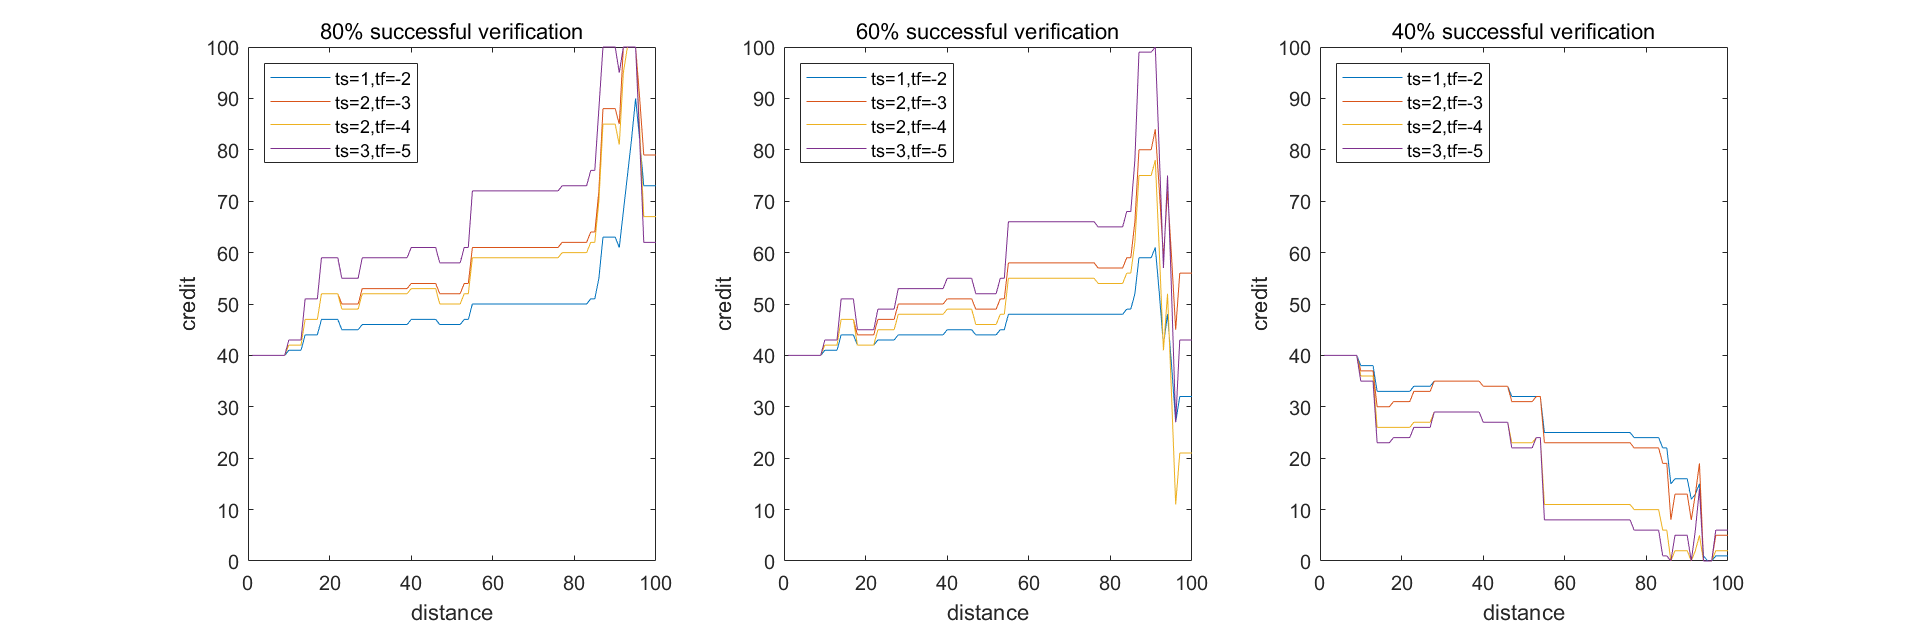
\includegraphics[width=1\linewidth]{figures/theta_num_total.png}
  \caption{给定验证成功率时,权重参数不同取值对应的信誉曲线}
  \label{fig:theta_num}
\end{figure}

\subsection{基于消息传播的信誉计算参数}
本节实验主要研究距离衰减系数$\gamma$对消息总评价的影响,主要通过调整收到消息的邻近车辆数、邻近车辆评价分布情况来确定合适的参数取值。实验中规定与目标车辆相距5个单位距离的车辆为收到消息并给出评价的邻近车辆,该群体的规模在5-15辆车之间;每辆车给出的评价为$[1,10]$之间的整数。同时,为了研究车辆距离与评价分布对总评价的影响,实验进一步规定了,与目标车辆相距2个单位距离及以内的车辆为中心车辆,其余车辆为边缘车辆。实验模拟了三种消息评价的分布模式:所有车辆给出的评价值都在$[1,10]$之间完全随机;中心车辆评价普遍高于边缘车辆(中心车辆打分集中在$[5,10]$,边缘车辆打分集中在$[1,6]$);中心车辆评价普遍低于边缘车辆(中心车辆打分集中在$[1,6]$,边缘车辆打分集中在$[5,10]$)。一次模拟按规则生成交互群体与交互结果,并根据算法计算得到消息的总评价;对于每组确定的邻近车辆数和分布模式,实验重复1000次模拟,记录消息总评价的平均值,结果如图4.5所示。

\begin{figure}
  \centering
  \subcaptionbox{随机评价\label{fig:gammarand}}
    {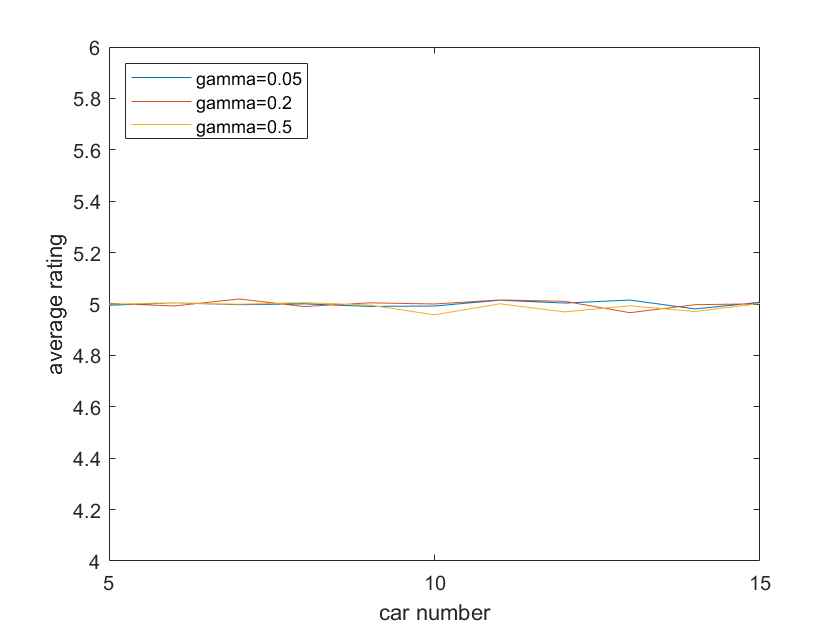
\includegraphics[width=0.49\linewidth]{figures/gamma_random.png}}
  \subcaptionbox{中心评价高于边缘评价\label{fig:gammahi}}
    {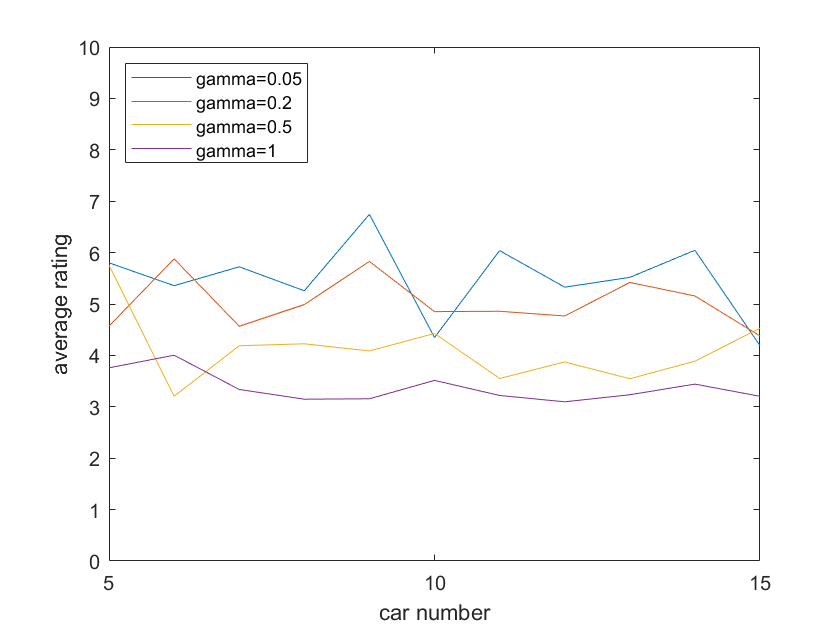
\includegraphics[width=0.49\linewidth]{figures/gamma_centerhi.png}}
    \subcaptionbox{中心评价低于边缘评价\label{fig:gammalo}}
    {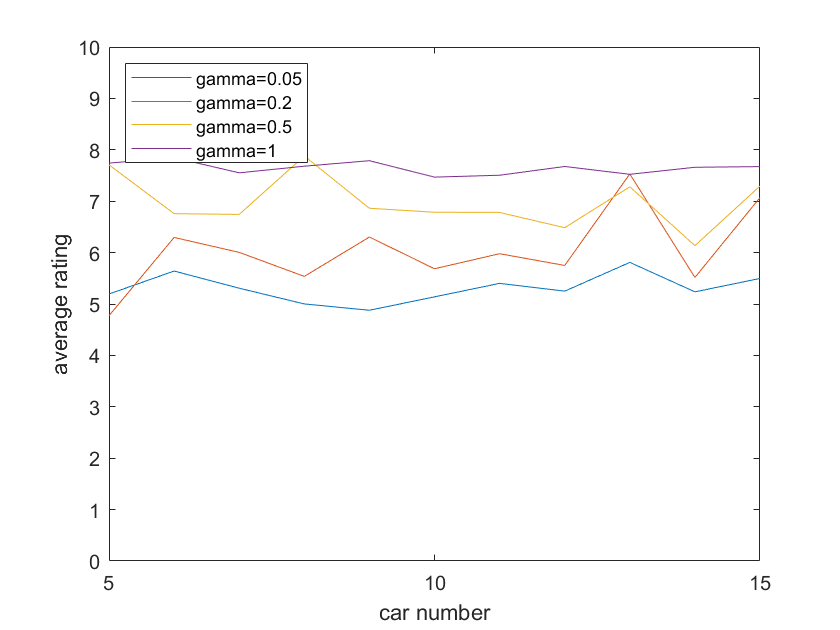
\includegraphics[width=0.49\linewidth]{figures/gamma_centerlo.png}}
  \caption{不同$\gamma$值在三种评价分布模式下对应的消息总评价均值}
  \label{fig:gamma}
\end{figure}

三张子图分别对应三种不同的消息评价分布,每张子图中,横坐标为邻近车辆的数量,纵坐标为消息总评价的均值,不同颜色的曲线分别对应参数$\gamma$的不同取值。从图~\ref{fig:gammarand}可以看出,在评价分布完全随机的情况下,车辆群体大小、$\gamma$取值对消息总评价在整体上几乎没有影响,其均值稳定在5分。图\ref{fig:gammahi}、图\ref{fig:gammalo}中消息评价均值随车辆群体规模的波动相对更大,但也是随机的,可以认为该因素对评价结果没有指向性的影响;同时容易看到,在中心车辆与边缘车辆给出评价相差较大时,$\gamma$取值越小,总评价在整体上就越偏向于中心车辆给出的评价。

图~\ref{fig:gammaerr}展示了后两种评价分布情况下,消息总评价在1000次模拟中的最大最小值。不完全随机的评价导致的数据波动幅度显然比完全随机要更大,$\gamma$取值较大时,周边车辆群体大小导致的数据波动下降,但是对于相同数量的群体来说,极端情况下给出的评价与平均值之间的差距要稍大一些。考虑到车辆距离与评价准确性之间的关系(中心车辆的评价通常来说比外围车辆更有说服力),以及数据的波动、稳定性等因素,选择较小的距离衰减系数$\gamma=0.2$。

\begin{figure}
  \centering
  \subcaptionbox{中心评价高于边缘评价\label{fig:gammahie}}
    {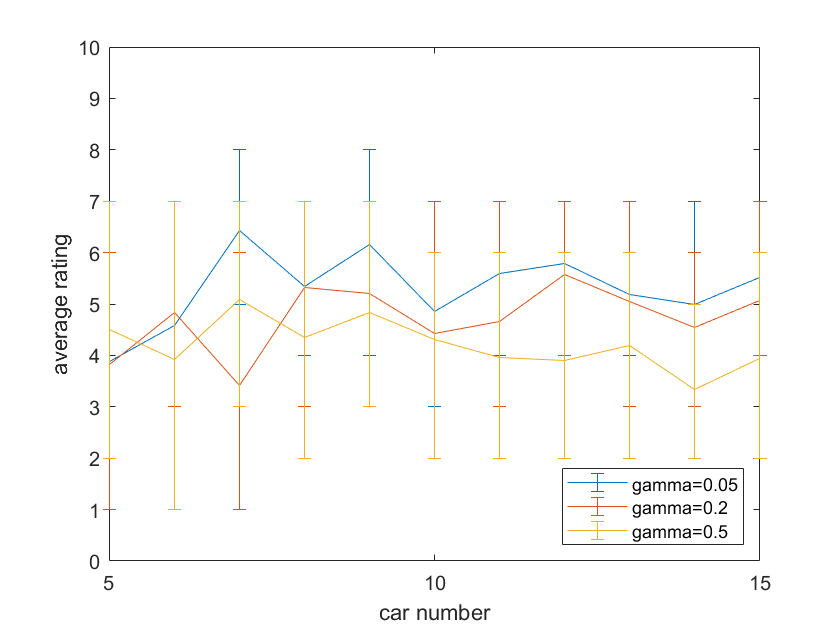
\includegraphics[width=0.49\linewidth]{figures/gamma_centerhi_err.png}}
  \subcaptionbox{中心评价低于边缘评价\label{fig:gammaloe}}
    {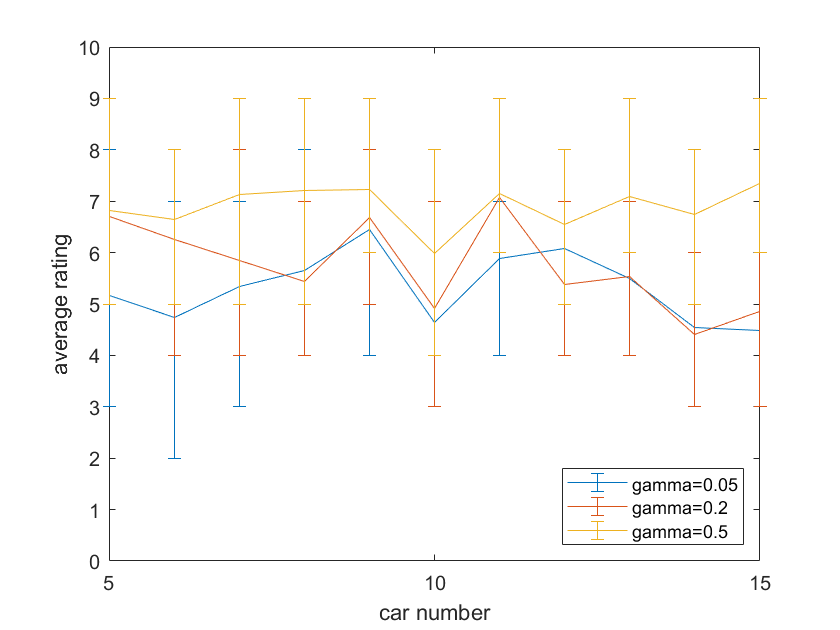
\includegraphics[width=0.49\linewidth]{figures/gamma_centerlo_err.png}}
  \caption{不同$\gamma$值在两种评价分布模式下对应的消息总评价均值与最值}
  \label{fig:gammaerr}
\end{figure}

从以上结果可以看到,消息总评价在统计学上整体向中心靠拢,但同时存在较大的波动空间,其具体结果还依具体情况而定。由于算法需要为信誉值确定一个判定消息是否可信的标准,依据消息总评价$Cred_m$划分可信区间如下:

\begin{equation*}
    \begin{aligned}
        &1\leq Cred_m\leq 5,\ \mbox{消息不可信,信誉值减小} \\
        &5< Cred_m\leq 6,\ \mbox{中立,信誉值不变} \\
        &6< Cred_m\leq 10,\ \mbox{消息可信,信誉值增加}
    \end{aligned}
\end{equation*}
写成公式:6-10:可信,信誉值增加;5-6:中立,信誉值不变;1-5:不可信,信誉值减小。

将消息评价的可信区间按此方式划分,是基于本节模拟实验的结果,考虑到完全随机的情况下评价均值统一趋近于5分,可以认为该分数对应着相对平均、难以判定正负的中立情况,而将中立区间设置得相对偏高,则是考虑到了对于不诚实消息传播者应当基于更严厉的评判标准。

\section{参数选取结果}

根据以上模拟测试与分析,确定信誉算法的相关参数为:

\begin{equation*}
    \begin{aligned}
        \delta&=0.2 \\
        \theta_{s}=2&,\ \theta_{f}=-3 \\
        \gamma=0.2,\ C_0&=5,\ C_1=6
    \end{aligned}
\end{equation*}

该组参数的选取确保了系统对于用户提交数据时间以及具体交互结果的敏感度,在智能合约进行小数截断的情况下,系统对每次交互都能产生较为明显的反馈;同时,尽量保证了在数据提交频繁的情况下,信誉值依然维持在合理的波动范围内,以避免在车辆极其密集的场景中,该评估结果由于产生极端的大幅波动而失去参考价值。该组参数在系统综合测试中的整体表现将在第5章中得到详细的描述与分析。

\section{本章小结}
本章利用原型系统设计了一系列实验,对信誉算法的参数取值进行了测试与分析。通过模拟实验,本章分别对算法中时间衰减系数、位置验证、消息传播几部分相关的参数进行了调优,从系统对时间和交互失败结果的敏感度、信誉整体走势、数据波动性等方面进行评价,并且最终确定了合适的参数值。